%% RSAA THESIS 'TEMPLATE' BY JOSHUA RICH <joshua.rich@gmail.com>
%% README:
% This template is designed to be used with pdflatex rather than plain
% latex.  It was developed under a TeXLive 2007 TeX distribution on
% Linux.  

% for requirements of typesetting and formatting see:
% http://info.anu.edu.au/Policies/_REG/Guidelines/PhD_Exam_Theses.asp
% (in emacs, type M-x browse-url with the cursor on 
% the link above)

%%NOTES ABOUT THE DOCUMENT CLASS
% Yes, I'm using a report style.  Any 'thesis style' you might
% find or someone will give you is based on the standard report
% class, but is probably well outdated compared to whatever TeX
% you have installed.  Besides, why use that style file if you 
% have no idea what it actually does?  You will probably just redefine
% all of its customisations anyway...
\documentclass[11pt,openright]{report} 

% define some constants that can be used in various places to easily
% specify title, subjects, author etc.
\newcommand{\thesistitle}{Type Ia Supernovae:
	Explosions and Progenitors}
\newcommand{\fullname}{Wolfgang Eitel Kerzendorf}
\newcommand{\shortname}{W. E. Kerzendorf}
\newcommand{\thesissubjects}{supernova:progenitors ????add some more?????}

%%NOTES ABOUT BABEL PACKAGE:
% It requires two components; the 
% \usepackage line above and the language put in the \documentclass.
% 'british' is used because that is the english style required for an
% ANU thesis.  This will ensure LaTeX uses british hyphenation and
% other language constructs when generating the text.  Putting the
% babel usepackage at the very top also ensures other packages called
% through \usepackage can take advantage of babel if they are set up
% for such.  
% We can also do tricky things in our ~/.emacs file if we
% are an emacs user now as well.  Grab the flyspell-babel and
% ispell-multi  emacs packages from:
% http://www.dur.ac.uk/p.j.heslin/Software/Emacs/
% And put it somewhere Emacs can find it (probably under ~/.emacs.d).
% Then add the following lines to your .emacs:
%   (dolist (hook '(LaTeX-mode-hook))
%   (add-hook hook (lambda () (flyspell-mode 1))))
%   (add-hook 'tex-mode-hook (function (lambda () (setq ispell-parser 'tex))))
%   (autoload 'flyspell-babel-setup "flyspell-babel")
%   (add-hook 'latex-mode-hook 'flyspell-babel-setup)
% After this, you should have Emacs auto-suggesting word corrections
% AND doing it in british-english automagically.  You can do a similar trick
% for papers by simply changing 'british' above to 'american', and
% flyspell will check your paper in american-english.
\usepackage[british]{babel}

%\usepackage{hyperref}

% ---------------------------------------------------------------------
% page size and margins
% ---------------------------------------------------------------------
%%NOTES ABOUT GEOMETRY PACKAGE:
% Below is using the geometry package as it is just cool.  This allows
% you to directly specify the margin requirements as outlined by ANU
% directly.  Here the inner border is 4cm and the outer is 2cm.  Top
% and bottom are also 2cm.  This is much easier than trying to work
% out page and margin dimensions by hand.  This is how you should use
% LaTeX...
\usepackage{geometry}
\geometry{a4paper,twoside}
\geometry{includehead,includefoot}
\geometry{hmargin={4cm,2cm}}
\geometry{vmargin={2cm,2cm}}

% ---------------------------------------------------------------------
% miscellaneous packages used
% ---------------------------------------------------------------------
\usepackage[hiresbb]{graphicx}
\DeclareGraphicsExtensions{.pdf}
%\DeclareGraphicsExtensions{.eps}
\usepackage[twoside]{rotating}

%%NOTES ABOUT FONTS PACKAGES:
% The basic requirements for fonts in an ANU thesis demand clear
% readability and that is about all.  So if you choose a nice,
% standard serif font you won't have any problems.
% I several font families in my thesis below:
%  pxfonts: math typesetting
%  tgpagella: for the normal text font (serif)
%  tgheros: for the sans serif font
%  tgcursor: for the typewriter style font
% TeX Gyre Pagella, Heros and Cursor are part of the TeX Gyre family
% of fonts, which can be obtained from:
%   http://www.gust.org.pl/projects/e-foundry/tex-gyre/
% Not all of the TeX Gyre, and possibly not the latest glyphs are
% available in standard TeX distributions.  
%
% The 'mathpazo' package provides an almost identical, albeit not
% actively developed font family to TeX Gyre Pagella and is included
% in standard TeX distributions.  This package
% also provides a full range of math glyphs.  You'd need to find
% alternative sans serif and typewriter fonts to use with this package.
%
% You can see a whole heap of LaTeX fonts, most of which are also in a
% standard TeX distribution at: 
%  http://www.tug.dk/FontCatalogue/
% This web-page shows what each font looks like and what you need to
% do to include the font in your document.  Note it lists fonts that
% may not be installed by your default TeX installation...
%
% Another list of fonts, recommended by `typophiles' can be found at:
%  http://typophile.com/node/18207
% Although the above list includes some really nice fonts, their
% availability in TeX distributions varies.  You may have to install
% them manually...
\usepackage[T1]{fontenc}
\usepackage{textcomp}
\usepackage{ucs}
\usepackage[utf8x]{inputenc}
\usepackage{amsmath,amssymb}
\usepackage{pxfonts}
\usepackage{tgheros,tgpagella}
\renewcommand*\ttdefault{qcr}
\linespread{1.05} % tgpagella/mathpazo need a bigger line spacing
\usepackage{microtype}
% bibliography uses natbib, this will be a requirement
\usepackage[round]{natbib}
% Super-nice looking tables, better than deluxetable
\usepackage{longtable,booktabs,multirow,ctable}

%%NOTES ABOUT CAPTION AND SUBFIG PACKAGES
% I'm using the caption package to style my captions.
% You need to read the documentation for this package (on CTAN) as it
% has simple explanations of the options and examples of what it looks
% like.
%
% The subfig package allows the ability to control in detail
% positioning of sub-plots in a complex figure as well as add labels
% to them, which can then be referenced in the text without the need
% for changing the actual number as your sub-figures change.
% The subfig package inherits options from the caption package, so
% declare them together.
%
\usepackage[]{caption,subfig}
\captionsetup{format=hang,%
  indention=-1.5cm,%
  labelsep=quad,%
  labelfont={footnotesize,bf},%
  textfont={footnotesize}}
% The hyperref package is a must while editing.  It provides urls
% inside your document; you can then click to go to certain pages,
% figures or bibliography entries.
\usepackage[unicode,pageanchor,colorlinks,plainpages=false]{hyperref}
% \hypersetup{pdftitle=\thesistitle\ - \shortname,%
%   pdfauthor=\fullname,%
%   pdfsubject={\thesissubjects},%
%   citecolor=DodgerBlue3,%
%   linkcolor=Ivory4,%
%   anchorcolor=CadetBlue4}
%for printing, make all colours black...
\hypersetup{pdftitle=\thesistitle\ - \shortname,%
pdfauthor=\fullname,%
pdfsubject={\thesissubjects},%
%citecolor=green,%
%filecolor=blue,%
%linkcolor=blue,%
%urlcolor=blue%
}
\usepackage{glossaries}
% Drop capitals at the start of chapters
\usepackage{lettrine}
% Allow defining of colours. Useful for:
% - defining the colours of links, citations etc.
% together with hyperref (i.e. in hyperrefsetup)
% - get alternating row colours or shades in tables
\usepackage[hyperref,x11names]{xcolor}
% Stops figures and tables 'floating' past the section in which they
% are declared.
\usepackage[section]{placeins}
\usepackage[toc,page,title,titletoc]{appendix}
%%NOTES ABOUT NAG
% this is a very good package to use.  If you want to write good LaTeX
% code and want to make sure you aren't using outdated methods (like
% your supervisor does), then use this package.  It will complain when
% you use outdated or wrong LaTeX commands.
\usepackage[l2tabu, orthodox]{nag}
\usepackage{ifthen}

% ---------------------------------------------------------------------
% styles for header, footer, pages, bibliography
% ---------------------------------------------------------------------
%

% chapter heading style
% this is the 'Conny' style from the fncychap package, modified to
% remove the two bold lines before the 'Chapter X' title.
% For usage of this package, see:
%  http://tug.ctan.org/cgi-bin/ctanPackageInformation.py?id=fncychap
%
\usepackage{fncychap}
\makeatletter
\ChNameUpperCase
\ChTitleUpperCase  
\ChNameVar{\centering\Huge\usefont{OT1}{qbk}{m}{n}\selectfont}
\ChNumVar{\Huge}
\ChTitleVar{\centering\Huge\usefont{OT1}{qbk}{m}{n}\selectfont}
\ChRuleWidth{2pt}
\renewcommand{\DOCH}{%
  \CNV\FmN{\@chapapp}\space \CNoV\thechapter
  \par\nobreak
  \vskip -0.5\baselineskip
}
\renewcommand{\DOTI}[1]{%
  \mghrulefill{\RW}\par\nobreak
  \CTV\FmTi{#1}\par\nobreak
  \vskip 60\p@
}
\renewcommand{\DOTIS}[1]{%
  \mghrulefill{\RW}\par\nobreak
  \CTV\FmTi{#1}\par\nobreak
  \vskip 60\p@
}

%
%%% page styles:
%
\usepackage{fancyhdr}
\fancyhead{}
\fancyfoot{}
%% make the odd pages have the section name on the top right
%\fancyhead[RO]{\usefont{OT1}{qbk}{m}{n}\selectfont \rightmark}
%% make the even pages have the chapter name on the top left
%\fancyhead[LE]{\usefont{OT1}{qbk}{m}{n}\selectfont \leftmark}
%
% fancy (main content) page header/footer styles
\fancyfoot[LE]{\usefont{OT1}{qbk}{m}{n}\selectfont \thepage}
\fancyfoot[RO]{\usefont{OT1}{qbk}{m}{n}\selectfont \thepage}
\renewcommand{\footrulewidth}{0.5pt}
\renewcommand{\footruleskip}{0mm}
% plain page header/footer styles (i.e. chapter pages)
\fancypagestyle{plain}{
\fancyhf{}
\fancyfoot[LE]{\usefont{OT1}{qbk}{m}{n}\selectfont \thepage}
\fancyfoot[RO]{\usefont{OT1}{qbk}{m}{n}\selectfont \thepage}
\renewcommand{\headrulewidth}{0pt}
\renewcommand{\footrulewidth}{0pt}
}

%
% this next section (till \makeatother) makes sure that blank pages
% are actually completely blank, cause they're not usually
\makeatletter
\def\cleardoublepage{\clearpage\if@twoside \ifodd\c@page\else
	\hbox{}
	\vspace*{\fill}
	\thispagestyle{empty}
	\newpage
	\if@twocolumn\hbox{}\newpage\fi\fi\fi}
\makeatother

%
%%% section header styles:
%
\usepackage[calcwidth]{titlesec}
\titlelabel{\thetitle.\quad}


%\includeonly{macros,chapter1}
%\includeonly{macros,chapter2}
%\includeonly{macros,chapter3}
%\includeonly{macros,chapter4}

% uncomment if you would like an index (make sure you actually define
% index terms in your document as well...
%\makeindex

% this contains various command definitions and other misc. options
% ---------------------------------------------------------------------
% command re-definitions and additions
% ---------------------------------------------------------------------

% i.e. -- e.g. -- etc. -- et. al.
\newcommand{\eg}{{\em e.g.,}}
\newcommand{\ie}{{\em i.e.,}}
\newcommand{\etc}{{\em etc.}}
\newcommand{\etal}{{\em et al.}}

% symbols
\newcommand{\HI}{\hbox{\rmfamily H\,{\textsc i}}}
\newcommand{\HIfat}{\hbox{\rmfamily\bfseries H\,{\textsc i}}}
\newcommand{\HIsub}{\hbox{{\scriptsize H}\,{\tiny I}}}
\newcommand{\HII}{\hbox{\rmfamily H\,{\scshape ii}}}
\newcommand{\HIIsub}{\hbox{\scriptsize \rmfamily H\,{\scshape ii}}}
\newcommand{\Ha}{\hbox{\rmfamily H\,$\alpha$}}
\newcommand{\msun}{\hbox{$M_{\odot}$}}
\newcommand{\mhi}{\hbox{$M_{\HIsub}$}}
\newcommand{\lsun}{\hbox{$L_{\odot}$}}
\newcommand{\mlsun}{(M/L)_{\odot}}
\newcommand{\vexp}{\hbox{$V_{exp}$}}
\newcommand{\vhel}{\hbox{$V_{hel}$}}
\newcommand{\vdisp}{\hbox{$\sigma_{disp}$}}
\newcommand{\Nhi}{\hbox{$N_{\HIsub}$}}
\newcommand{\nhi}{\hbox{$n_{\HIsub}$}}
\newcommand{\Mhi}{\hbox{$M_{\HIsub}$}}
\newcommand{\ra}{$\alpha$}
\newcommand{\dec}{$\delta$}
\newcommand{\degree}{\textdegree}
\newcommand{\arcmin}{\hbox{$^\prime$}}
\newcommand{\arcsec}{\hbox{$^{\prime\prime}$}}
\newcommand{\kms}{\hbox{km s$^{-1}$}}
\newcommand{\mjbeam}{\hbox{mJy beam$^{-1}$}}
\newcommand{\jbeam}{\hbox{Jy beam$^{-1}$}}
\newcommand{\mjbeamkms}{\hbox{mJy/beam km s$^{-1}$}}
\newcommand{\jkms}{\hbox{Jy km s$^{-1}$}}
\newcommand{\coldensity}{\hbox{cm$^{-2}$}}
\newcommand{\voldensity}{\hbox{cm$^{-3}$}}
% add others you need

% footnote symbols
% use \symbolfootnote[1]{footnote} to get an *
%     * 1 - *
%     * 2 - dagger
%     * 3 - double dagger
%     * 4 - ... 9 (see page 175 of the latex manual) 
\long\def\symbolfootnote[#1]#2{\begingroup%
\def\thefootnote{\fnsymbol{footnote}}\footnote[#1]{#2}\endgroup}
% New definition of square root:
% it renames \sqrt as \oldsqrt
% it defines the new \sqrt in terms of the old one
% See:
%  http://en.wikibooks.org/wiki/LaTeX/Tips_and_Tricks#New_Square_Root
\let\oldsqrt\sqrt
\def\sqrt{\mathpalette\DHLhksqrt}
\def\DHLhksqrt#1#2{%
\setbox0=\hbox{$#1\oldsqrt{#2\,}$}\dimen0=\ht0
\advance\dimen0-0.2\ht0
\setbox2=\hbox{\vrule height\ht0 depth -\dimen0}%
{\box0\lower0.4pt\box2}}
% define a new url command so a nice font can be used
\newcommand{\myurl}[1]{\small\texttt{#1}}
% handy referencing of figures/tables, see 'Guide to using Encapsulated
% PostScript in LaTeX.', Section 17.1.1
\newcommand\FigDiff[1]{\hyperref[#1]{Figure~\ref*{#1}} on Page~\pageref*{#1}}
\newcommand\FigSame[1]{\hyperref[#1]{Figure~\ref*{#1}}}
\newcommand\Figref[1]{\ifthenelse{\value{page}=\pageref{#1}}
                     {\FigSame{#1}}{\FigDiff{#1}}}
\newcommand\TabDiff[1]{\hyperref[#1]{Table~\ref*{#1}} on Page~\pageref*{#1}}
\newcommand\TabSame[1]{\hyperref[#1]{Table~\ref*{#1}}}
\newcommand\Tabref[1]{\ifthenelse{\value{page}=\pageref{#1}}
                     {\TabSame{#1}}{\TabDiff{#1}}}

% text to add to end of continued figures caption
\newcommand\ContFig[1]{\textit{(Figure continued from page \pageref*{#1})}}

% ---------------------------------------------------------------------
% pdflatex setup
% ---------------------------------------------------------------------
% make pdflatex use the same spacing (paragraph, line and page breaks)
% as standard LaTeX 
\pdfadjustspacing=1

% ---------------------------------------------------------------------
%  misc. options
% ---------------------------------------------------------------------
% table of contents will go to subsubsections
\setcounter{tocdepth}{3}  

% ---------------------------------------------------------------------
% more liberal 'float' (tables, figures) placement
% ---------------------------------------------------------------------
% Alter some LaTeX defaults for better treatment of figures:
% See p.105 of "TeX Unbound" for suggested values.
% See pp. 199-200 of Lamport's "LaTeX" book for details.
% General parameters, for ALL pages:
\renewcommand{\topfraction}{0.9}	% max fraction of floats at top
\renewcommand{\bottomfraction}{0.8}	% max fraction of floats at bottom
% Parameters for TEXT pages (not float pages):
\setcounter{topnumber}{2}
\setcounter{bottomnumber}{2}
\setcounter{totalnumber}{4}     % 2 may work better
\setcounter{dbltopnumber}{2}    % for 2-column pages
\renewcommand{\dbltopfraction}{0.9}	% fit big float above 2-col. text
\renewcommand{\textfraction}{0.07}	% allow minimal text w. figs
% Parameters for FLOAT pages (not text pages):
\renewcommand{\floatpagefraction}{0.7}	% require fuller float pages
% N.B.: floatpagefraction MUST be less than topfraction !!
\renewcommand{\dblfloatpagefraction}{0.7}	% require fuller float pages
% remember to use [htp] or [htpb] for placement

% ---------------------------------------------------------------------
% Journal name abbreviations
% ---------------------------------------------------------------------
\newcommand{\jnlref}[1]{\textrm{#1}}
\newcommand{\aj}{\jnlref{AJ}}
\newcommand{\araa}{\jnlref{ARA\&A}}
\newcommand{\apj}{\jnlref{ApJ}}
\newcommand{\apjl}{\jnlref{ApJ}}
\newcommand{\apjs}{\jnlref{ApJS}}
\newcommand{\ao}{\jnlref{Appl.~Opt.}}
\newcommand{\apss}{\jnlref{Ap\&SS}}
\newcommand{\aap}{\jnlref{A\&A}}
\newcommand{\aapr}{\jnlref{A\&A~Rev.}}
\newcommand{\aaps}{\jnlref{A\&AS}}
\newcommand{\azh}{\jnlref{AZh}}
\newcommand{\baas}{\jnlref{BAAS}}
\newcommand{\jrasc}{\jnlref{JRASC}}
\newcommand{\memras}{\jnlref{MmRAS}}
\newcommand{\mnras}{\jnlref{MNRAS}}
\newcommand{\pra}{\jnlref{Phys.~Rev.~A}}
\newcommand{\prb}{\jnlref{Phys.~Rev.~B}}
\newcommand{\prc}{\jnlref{Phys.~Rev.~C}}
\newcommand{\prd}{\jnlref{Phys.~Rev.~D}}
\newcommand{\pre}{\jnlref{Phys.~Rev.~E}}
\newcommand{\prl}{\jnlref{Phys.~Rev.~Lett.}}
\newcommand{\pasp}{\jnlref{PASP}}
\newcommand{\pasj}{\jnlref{PASJ}}
\newcommand{\qjras}{\jnlref{QJRAS}}
\newcommand{\skytel}{\jnlref{S\&T}}
\newcommand{\solphys}{\jnlref{Sol.~Phys.}}
\newcommand{\sovast}{\jnlref{Soviet~Ast.}}
\newcommand{\ssr}{\jnlref{Space~Sci.~Rev.}}
\newcommand{\zap}{\jnlref{ZAp}}
\newcommand{\nat}{\jnlref{Nature}}
\newcommand{\iaucirc}{\jnlref{IAU~Circ.}}
\newcommand{\aplett}{\jnlref{Astrophys.~Lett.}}
\newcommand{\apspr}{\jnlref{Astrophys.~Space~Phys.~Res.}}
\newcommand{\bain}{\jnlref{Bull.~Astron.~Inst.~Netherlands}}
\newcommand{\fcp}{\jnlref{Fund.~Cosmic~Phys.}}
\newcommand{\gca}{\jnlref{Geochim.~Cosmochim.~Acta}}
\newcommand{\grl}{\jnlref{Geophys.~Res.~Lett.}}
\newcommand{\jcp}{\jnlref{J.~Chem.~Phys.}}
\newcommand{\jgr}{\jnlref{J.~Geophys.~Res.}}
\newcommand{\jqsrt}{\jnlref{J.~Quant.~Spec.~Radiat.~Transf.}}
\newcommand{\memsai}{\jnlref{Mem.~Soc.~Astron.~Italiana}}
\newcommand{\nphysa}{\jnlref{Nucl.~Phys.~A}}
\newcommand{\physrep}{\jnlref{Phys.~Rep.}}
\newcommand{\physscr}{\jnlref{Phys.~Scr}}
\newcommand{\planss}{\jnlref{Planet.~Space~Sci.}}
\newcommand{\procspie}{\jnlref{Proc.~SPIE}}
\newcommand{\ieeesigprocm}{\jnlref{IEEE~Signal~Processing~Magazine}}
\newcommand{\cjaa}{\jnlref{Chinese J. Astron. Astrophys.}}
\let\astap=\aap
\let\apjlett=\apjl
\let\apjsupp=\apjs
\let\applopt=\ao

%%% Local Variables:
%%% TeX-master: "thesis.tex"
%%% End:


\begin{document}

% !TEX root = ../thesis.tex
\chapter{Linear interpolation in N~Dimensions}
\label{chap:ndinterp}

Interpolation is one of the most common operations in astronomy. Resampling spectra to a different wavelength grid, projecting images or interpolating physical quantities in n-dimensional fluid dynamics simulation are all examples of interpolation.
Interpolation can be described as a special case of curve fitting which requires the function to go through all points. 

In one dimension interpolation is relatively easy and there exist multiple methods. The simplest method is nearest-neighbour interpolation in which the algorithm picks the closest neighbour point to the point to be interpolated. 

Linear interpolation is one of the most common methods of interpolation. The two neighbouring points of the point to be interpolated are found and their slope and offset is used to obtain the interpolated point.

A more sophisticated approach is the spline-method of interpolation. Splines are piecewise polynomials of n-th degree whose first and second derivation are the same at the data points.

In one dimensional space there exists an abundance of interpolation methods. This multitude of options decreases rapidly with increasing number of dimensions. 
We will focus on the implementation of linear interpolation in N-dimensions, although there are a few other options like nearest neighbour interpolation and radial basis function.

For our linear interpolation we have opted to use \deltri\ as a interpolation method. The interpolation involves multiple steps to arrive at an interpolation solution: At first a \deltri\ is performed on the existing points. As a next step we need to find the simplex(geometric structure; a triangle in two dimensions) that contains the point to be interpolated. 
Finally we will use the barycentric coordinate system of the simplex to perform the actual interpolation.






\section{Delauney triangulation}
\label{sec:delauney_tri}
A triangulation is the process of connecting all points in a set with straight lines without any two lines crossing (see Figure \ref{fig:delauney_example}). It is obvious that there many ways for a set to be triangulated. All triangulations however have the same outer boundary called the convex hull. One special kind of triangulation is the \deltri. The \deltri\ can be defined a various abstract ways and has intriguing properties.

\begin{figure}[tb] %  figure placement: here, top, bottom, or page
   \centering
   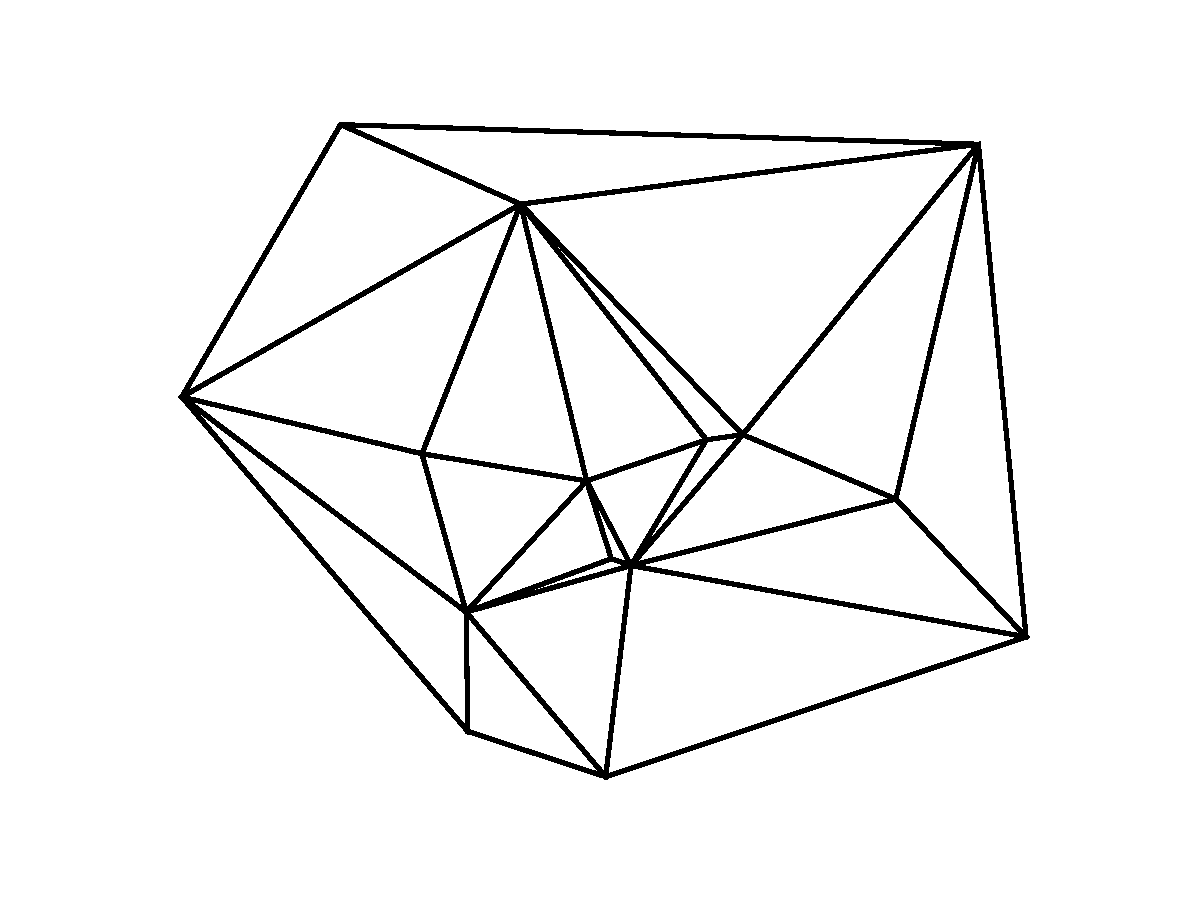
\includegraphics[width=\textwidth]{chapter_ndinterp/plots/simple_delauney.pdf} 
   \caption{\deltri\ of 20 points in two dimensions.}
   \label{fig:delauney_example}
\end{figure}

For a description of the process we will limit ourselves to two dimensions. This process is expandable to n dimensions in which the triangles become geometric structures called n-simplices.
One such defintion is that the circum-circle (circle going through all three points of the triangle) of each triangle must only contain three points. Figure \ref{fig:delauney_allowed}, a simple example, shows one \textit{legal} triangulation and one \textit{illegal} triangulation. One can see in the \textit{illegal} triangulation that the circum-circles of both triangles contain more than tree points. By doing a simple "\textit{edge-flip}" one arrives at the \deltri. In addition this ensures that the triangulation gives the largest minimum angle for both triangles. 

\begin{figure}[tb] %  figure placement: here, top, bottom, or page
   \centering
   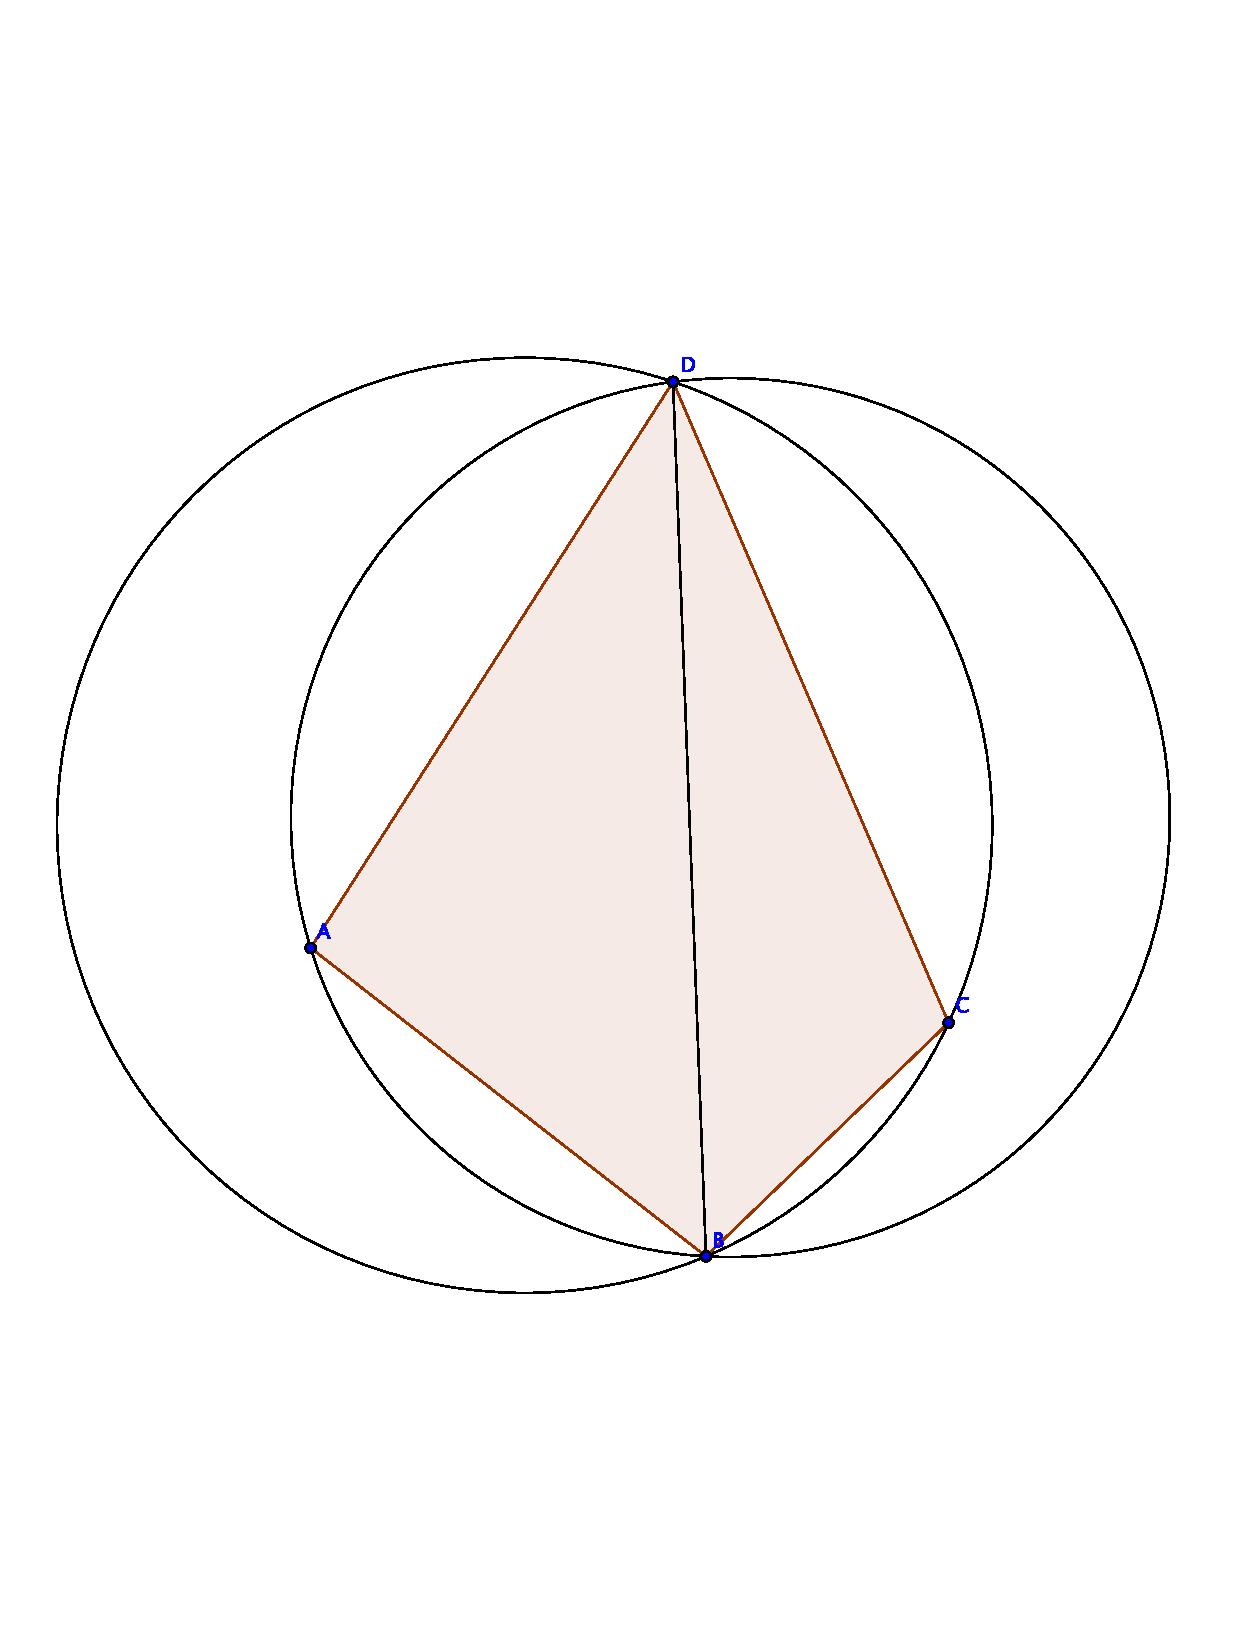
\includegraphics[width=.45\textwidth]{chapter_ndinterp/plots/illegal_triangulation.pdf} 
   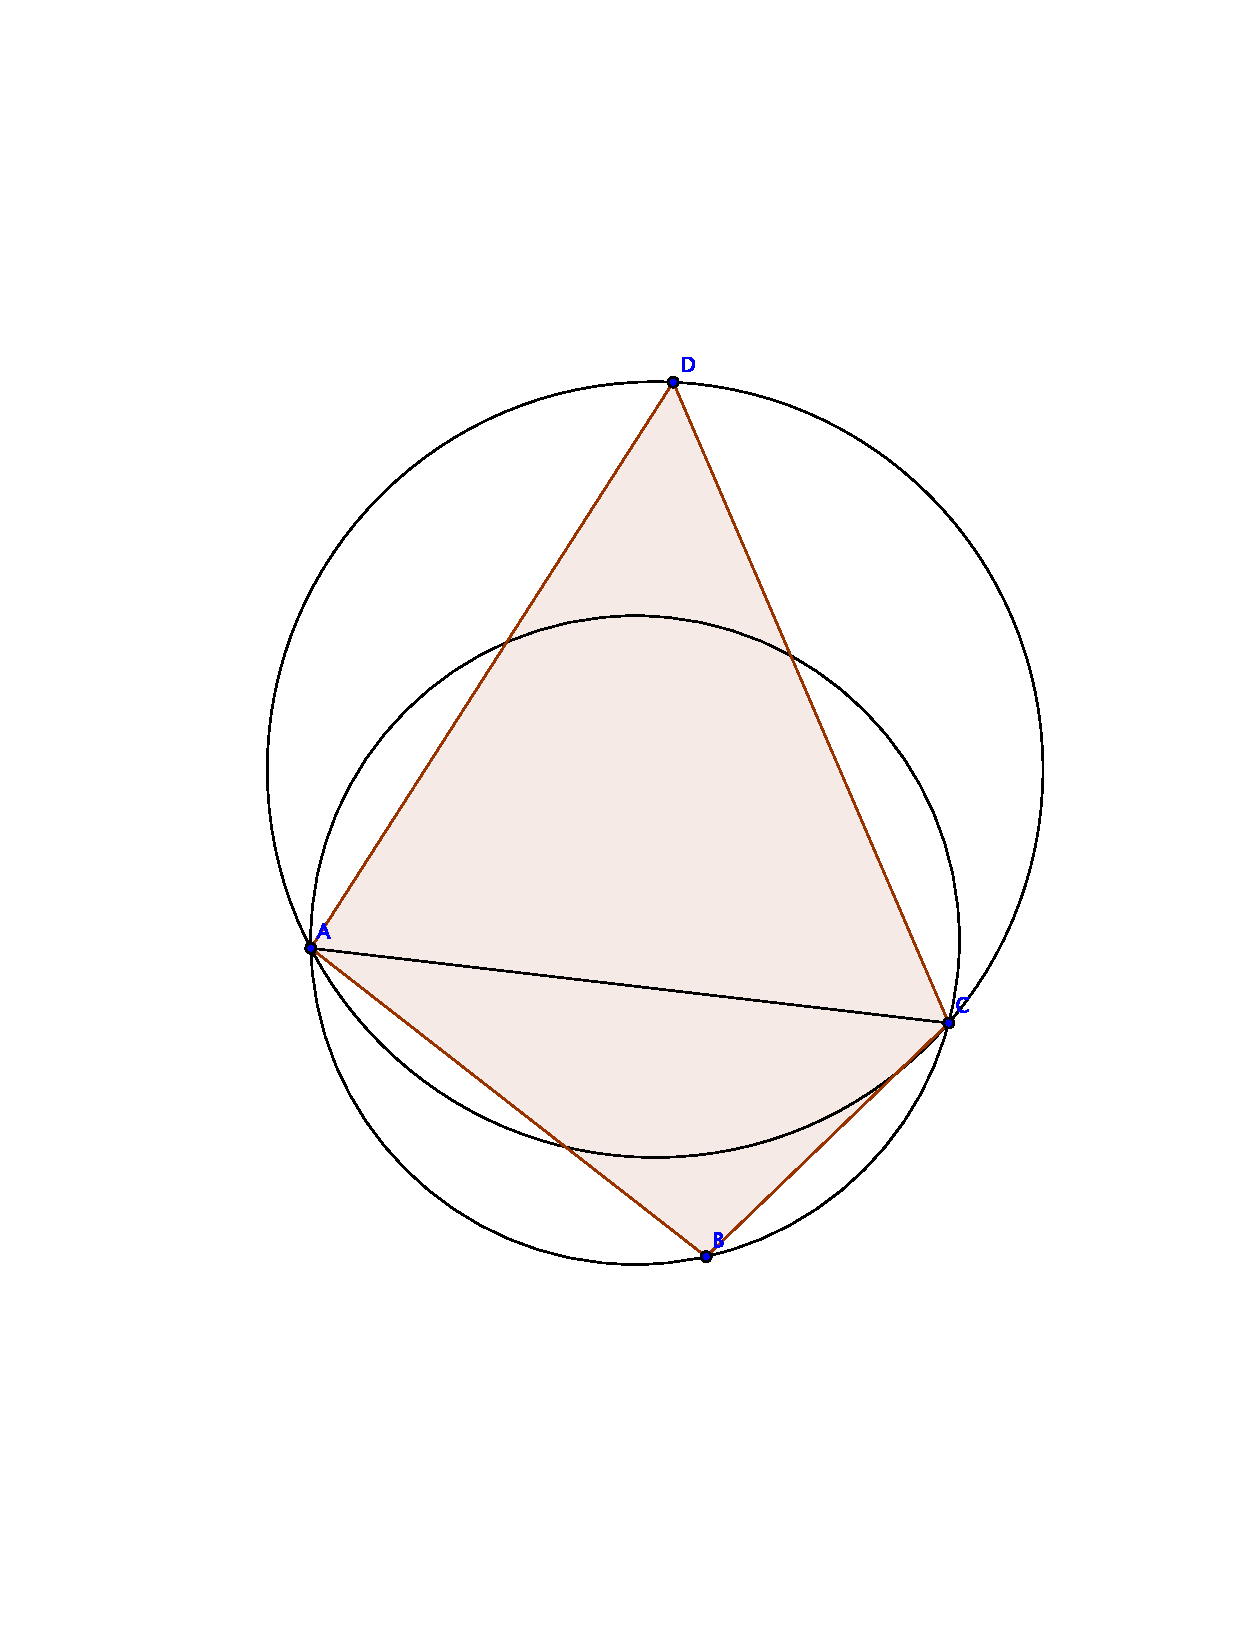
\includegraphics[width=.45\textwidth]{chapter_ndinterp/plots/edge_flip.pdf} 
   \caption[Change from a `illegal' triangulation to a \deltri]{The left figure shows an `\textit{illegal}' triangulation of the 4 points. Both circles include all the points. With a so called edge flip one can arrive at a `\textit{legal}' triangulation.}
   \label{fig:delauney_allowed}
\end{figure}
\deltri\ and convex hulls have a very interesting relation. It is possible construct the \deltri\ in n dimensions from a convex hull of the points projected on a paraboloid in n+1 dimensions.
Figure \ref{fig:delauney_projection} shows an example of a \deltri\ in two dimensions constructed from the convex hull in three dimensions. To project the points onto the paraboloid one just square sums the coordinates n dimensions and uses this as the coordinate for the point in n+1 dimensions. 

\begin{figure}[tb] %  figure placement: here, top, bottom, or page
   \centering
   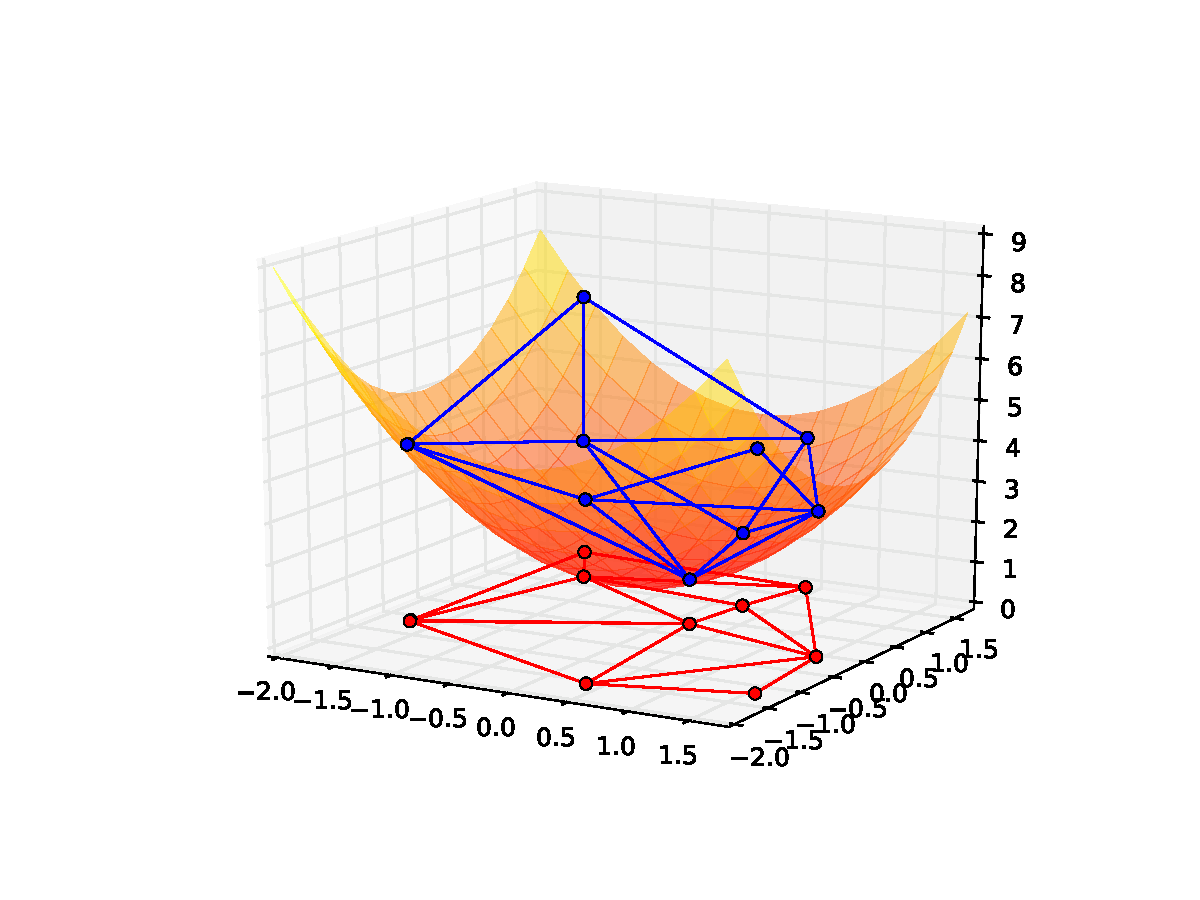
\includegraphics[width=0.49\textwidth]{chapter_ndinterp/plots/delauney_project_left.pdf} 
   \hspace{-1.5cm}
   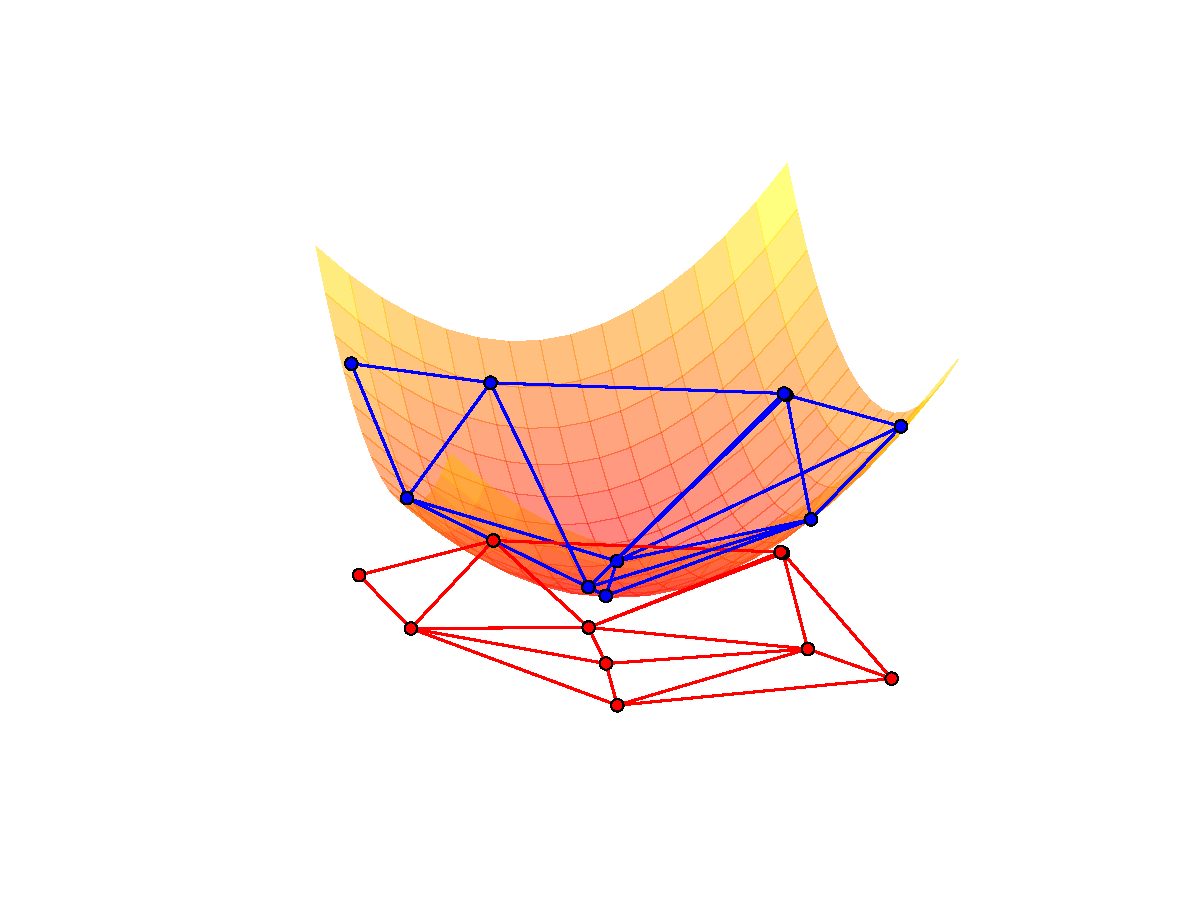
\includegraphics[width=0.49\textwidth]{chapter_ndinterp/plots/delauney_project_right.pdf} 
   \caption[Stereogram of the projection of the convex hull in three dimensions]{Stereogram \citep[produced using a method described in ][]{Vogt11} of the projection of the convex hull in three dimensions to form the \deltri\ in two dimensions.}
   \label{fig:delauney_projection}
\end{figure}

\section{Convex Hull}
In section \ref{sec:delauney_tri} we have described the relation between the convex hull  and the \deltri. There are multiple ways to construct the convex hull for N points, we will limit ourselves to the description of the Quickhull algorithm \citep{Barber96thequickhull}. Similar to the Quicksort algorithm it follows the divide and conquer strategy. 


\begin{figure}[tb] %  figure placement: here, top, bottom, or page
   \centering%
   \subfloat[Twenty points for which we are trying to find the convex hull.]{%
%   \missingfigure[figwidth=0.4\textwidth]{Test}%
   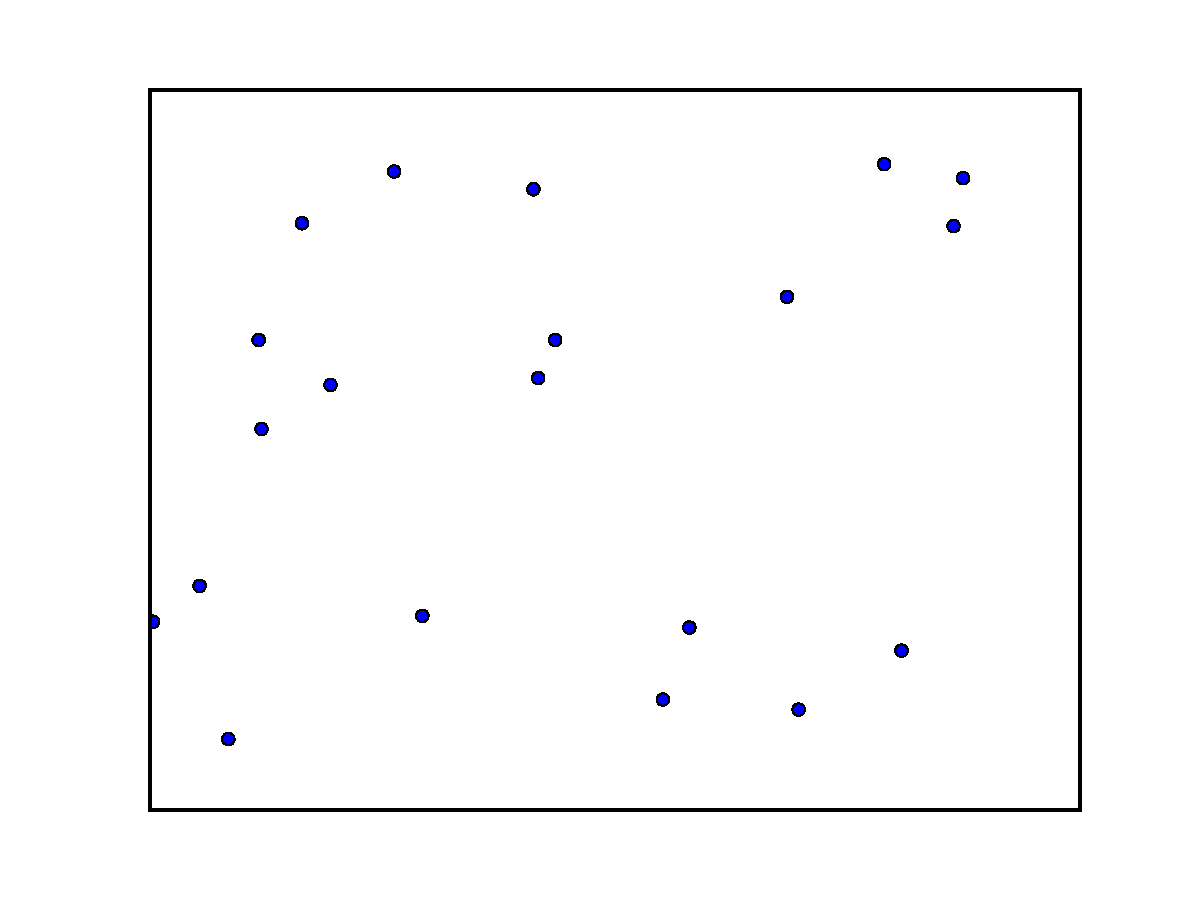
\includegraphics[width=0.4\textwidth]{chapter_ndinterp/plots/qhull_1.pdf}%
   \hfill
   \label{fig:qhull_1}%
 }\quad%
 \subfloat[We find the points with the lowest and highest x-value and connect them with a line.]{
%   \missingfigure[figwidth=0.4\textwidth]{Test}%
   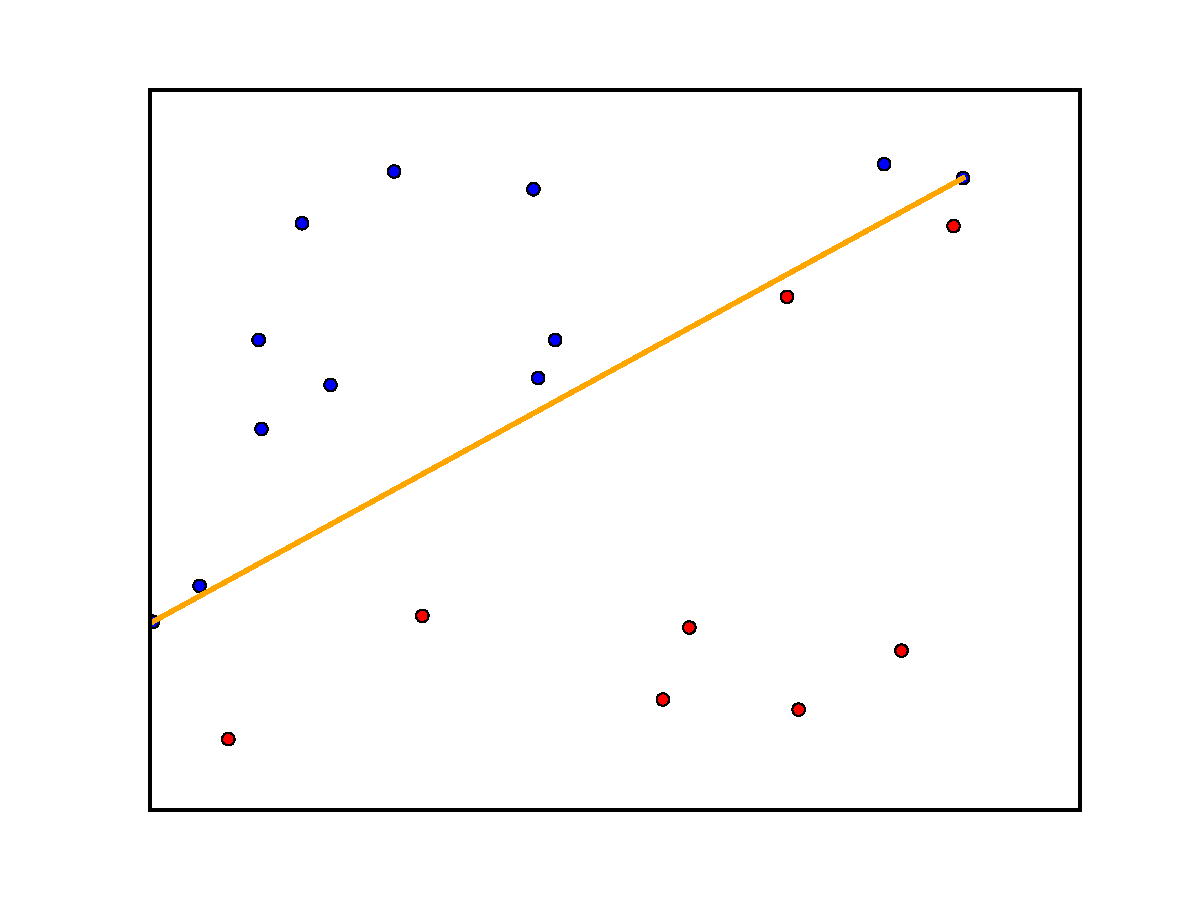
\includegraphics[width=0.4\textwidth]{chapter_ndinterp/plots/qhull_2.pdf}%
   \label{fig:qhull_2}%
 }\\%
 \subfloat[Continuing with the points on the left (same process happens recursively on the right) we find the point furthest away from the line. We then draw two more lines and build a triangle. The points inside of the triangle are not part of the convex hull and are discarded. We will repeat the current step with the two new lines of the triangle. ]{%
 %  \missingfigure[figwidth=0.4\textwidth]{Test}%
   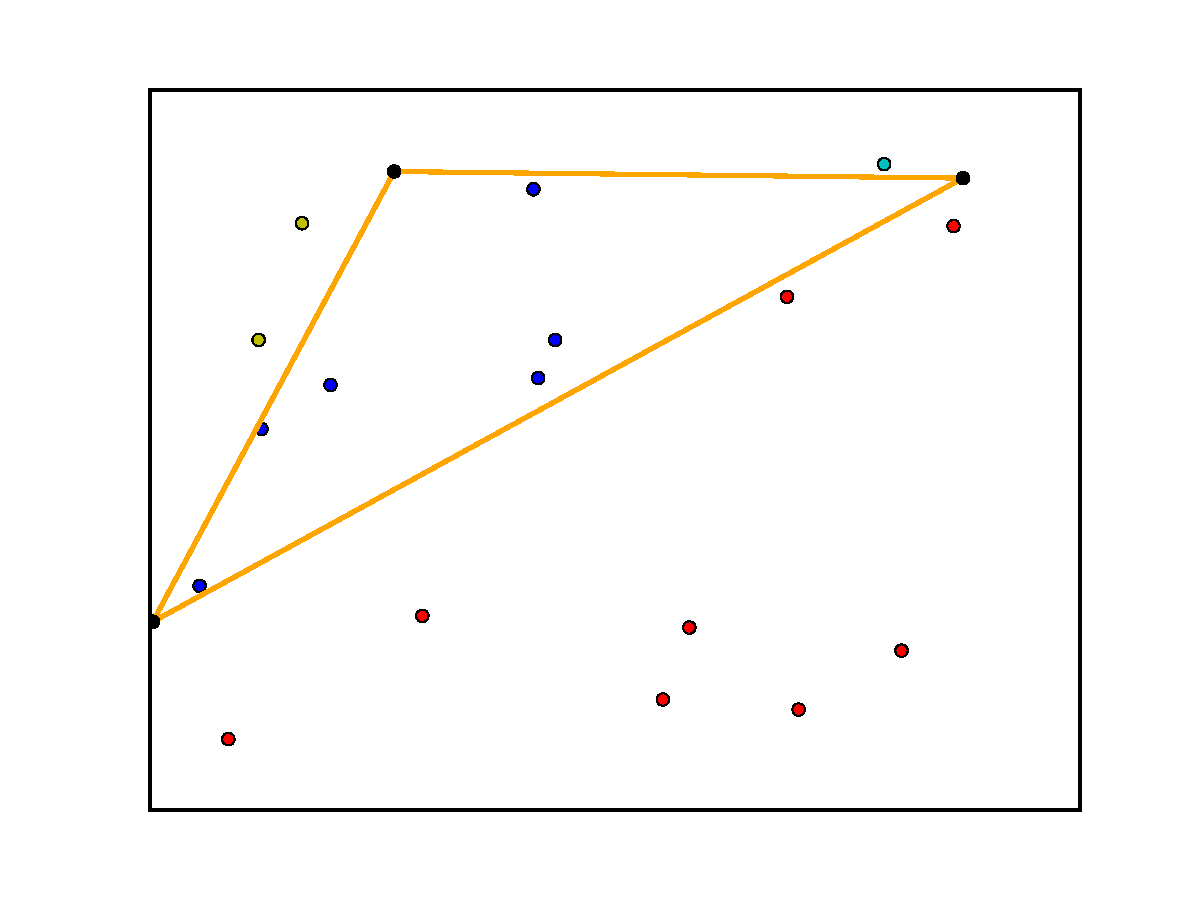
\includegraphics[width=0.4\textwidth]{chapter_ndinterp/plots/qhull_3.pdf}%
   \label{fig:qhull_3}%
 }\qquad%
 \subfloat[We have found points of the convex hull once we can't build a new triangle anymore.]{%
%   \missingfigure[figwidth=0.4\textwidth]{Test}%
   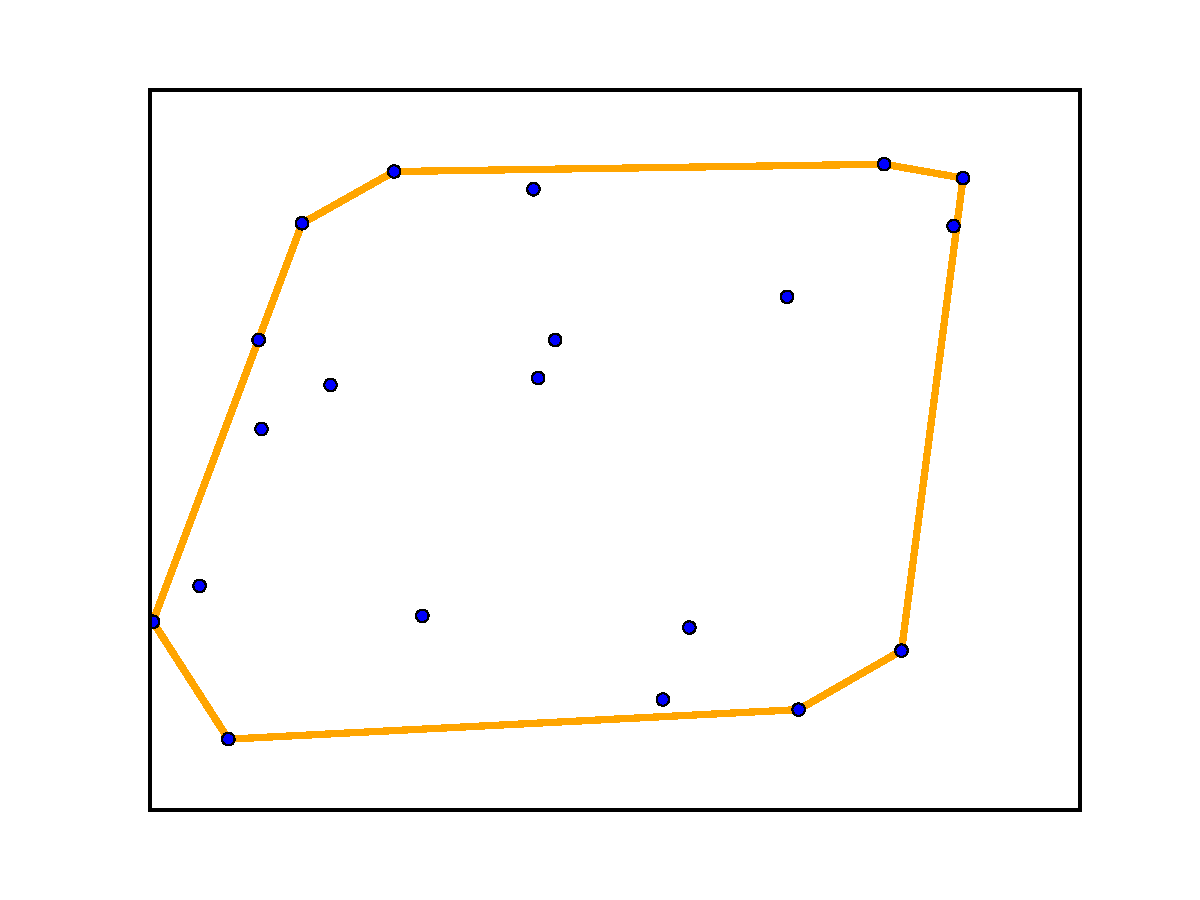
\includegraphics[width=0.4\textwidth]{chapter_ndinterp/plots/qhull_final.pdf}%
   \label{fig:qhull_4}%
 }\quad%
   \caption{Determination of a convex hull in two dimensions. }%
   \label{fig:example}%
\end{figure}%

As an initial input we have N data points. Although this method works in n-dimensions, we will show an example in two dimensions.
The first operation is finding the two extreme points in the horizontal axis, which are guaranteed to be part of the convex hull. 
We connect these two extreme points thus creating a division between a ``left'' and a ``right'' set of point. Now the divide and conquer method begins. We will only describe what happens to the left side, but imply that the same steps are taken on the right side. 
We find the point furthest away from the dividing line and add it. A triangle is formed out of the two points of the initial dividing line and the additional point. All points inside the triangle do not belong to the convex hull and thus we exclude them. The triangle again divides the remaining points into two sets, one left of the triangle and one right which are again iterated over recursively. 

The method is repeated until each subset only contains the start and end point of the dividing line. 
We have created the convex hull, which if projected to a $d - 1$-dimensional space provides the \deltri\ of the projected points. For this projection to work we need to construct a convex hull in more than two dimensions which uses the same technique as described.


\section{Barycentric coordinates system}

The actual interpolation transforms the interpolant's coordinate into the barycentric coordinates of the containing triangle.

One can construct the barycenter of a triangle by drawing lines from each point to the midpoint of the opposing side (see Figure \ref{fig:tri_barycenter}). 


\begin{figure}[htbp] %  figure placement: here, top, bottom, or page
   \centering
   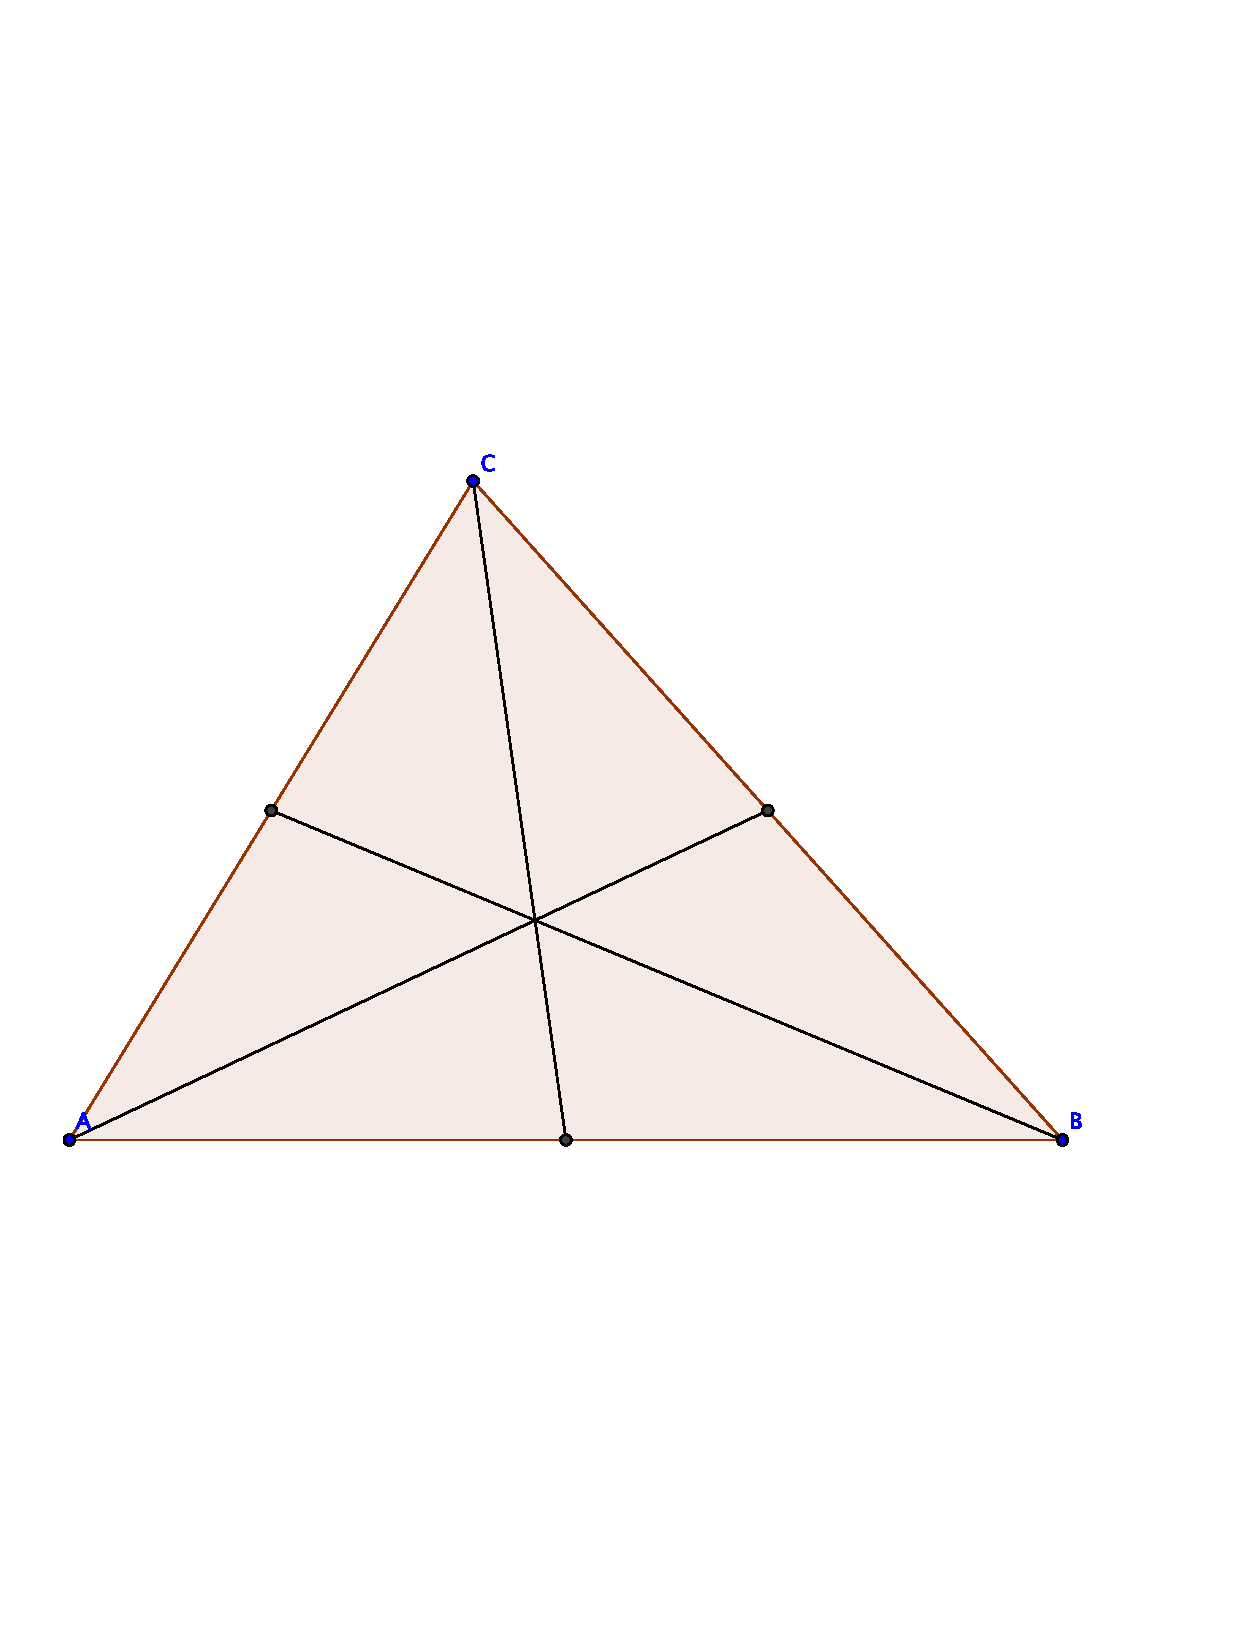
\includegraphics[width=0.7\textwidth]{chapter_ndinterp/plots/barycenter.pdf}
   \caption{The triangle and its barycenter marked by the intersection of lines. }
   \label{fig:tri_barycenter}
\end{figure}


The coordinates of the barycenter M can simply be expressed by,
\[
\vec{M} = \frac{1}{3} (\vec{A} + \vec{B} + \vec{C}).
\]

Not only the barycenter can be expressed by the vectors of $\vec{A}$, $\vec{B}$ and $\vec{C}$ but every point p inside the triangle can be expressed by,
\[
\vec{p} = \alpha\vec{A} + \beta\vec{B} + \gamma\vec{C},
\]
where
\[
\alpha + \beta + \gamma = 1.
\]
$\alpha$, $\beta$ and $\gamma$ are called the barycentric coordinates. If the point p lies within the triangle all barycentric coordinates are positive. 

\section{Triangle Finding and Interpolation}

To calculate the interpolation using barycentric coordinates we need to find the n-simplex that contains the interpolant. We use a method called directed walk (priv. comm. Pauli Virtanen).  We choose a random starting n-simplex. In order to interpolate to a given point (interpolant) we calculate the barycentric coordinates for the interpolant and test if all of them are larger than 0. In that case  we have found the n-simplex that contains the point. 
If the n-th barycentric coordinate is negative we jump to the neighbouring n-simplex which is opposite the n-th point. This is iterated until the containing n-simplex is found or the next jump would lead outside the convex hull of the \deltri. For the latter case the point is outside of the grid and can not be interpolated.

If this algorithm converges and the right n-simplex is found the interpolation can be easily performed using the barycentric coordinates:
\[
f(\vec{p})=\alpha f(\vec{A}) + \beta f(\vec{B}) + \gamma f(\vec{C})
\]
where  $\vec{A}$, $\vec{B}$ and $\vec{C}$ are the points of the triangle. 


\section{Conclusion}

We have described the method of linear interpolation using \deltri\ mainly in two dimensions. As mentioned this method is easily extensible to n dimensions. The triangles (3-simplices) become n-simplices in n dimensions (e.g. Tetrahedrons in three dimensions). The method itself however stays very similar for higher dimensions. 

In this work we have made extensive use of n-dimensional linear interpolation using the implementation present in the \gls{scipy} package, called \textsc{LinearNDInterpolator}. In this case creation of the convex-hull is performed by the QHULL implementation described in \citet{Barber96thequickhull}.

We have tested the performance of the algorithm by creating a three dimensional grid with $20\times10\times10$ gridpoints and an array of 10, 000  double values at each gridpoint. 
On a standard 2011 MacBook Pro (Intel Core i7, 2.6 GHz, running only on a single processor) we have measured the initial building of the \deltri and storing it in an appropriate data structure to 256\,ms. The interpolation for random points took on average $\approx600\,\mu$\,s. This technique lends itself very well to explore large datasets even on moderately equipped machines. 

We have used this technique extensively to interpolate a spectral grid in three dimension (\gls{teff}, \gls{logg}\ and \gls{feh}). When trying to extract stellar parameters from an input spectrum we calculated the $\chi^2$ for the observed spectrum with interpolated synthetic spectra from the grid. The interpolated spectra resulting from the interpolation are continuous, but not differentiable at the ridges of the grid structure (ridges are the borders of the simplices that make the grid). This non-differentiability at the ridges can be seen even in the $\chi^2$ space. Optimisers that employ gradient methods \citep[such as MIGRAD][]{James:1975dr} show some difficulties in some regions of the search space. We have tried to alleviate this problem by beginning the optimisation from different starting points. In almost all cases this lead to the same minimum.

In summary, the presented linear n-dimensional interpolator is a very robust and quick way to explore large parameter spaces without having to compute each single point. 

Future work will be directed to exploring other n-dimensional interpolators in the astrophysical context. 



%% !TEX root =../thesis.tex
\chapter{SN1006}
\label{chap:three}

\lettrine[lines=4]{L}{orem} ipsum dolor sit amet, consectetuer
adipiscing elit. Mauris posuere, elit ac suscipit pulvinar, purus
felis vehicula purus, sed pellentesque arcu nibh eu turpis. Vivamus
volutpat convallis mi. Aliquam varius magna eu urna lacinia
dignissim. Proin venenatis tellus. Fusce pede dui, semper varius,
venenatis vitae, ultrices ac, dolor. Proin diam. Suspendisse eget
purus id leo accumsan scelerisque. Integer rutrum. Etiam risus nibh,
auctor eu, eleifend id, interdum ut, odio. Suspendisse
potenti. Praesent ultricies, mauris convallis vestibulum viverra,
nulla risus porttitor tellus, ut consequat velit nunc at nisi. Nulla
rhoncus nisl quis urna. Morbi sed nunc at tortor rhoncus
iaculis. Lorem ipsum dolor sit amet, consectetuer adipiscing elit. Sed
augue. Nunc molestie.

Maecenas at lectus id nunc bibendum placerat. Suspendisse cursus,
magna vitae blandit bibendum, nisi justo facilisis mi, at faucibus
elit urna id felis. Lorem ipsum dolor sit amet, consectetuer
adipiscing elit. Maecenas risus erat, ornare ac, varius nec, molestie
sed, nulla. Praesent sem urna, sollicitudin in, vulputate at, suscipit
vehicula, lectus. Integer mollis. Curabitur ornare, erat a facilisis
sagittis, risus nulla faucibus diam, at vehicula justo magna nec
urna. Pellentesque rhoncus, turpis eu facilisis molestie, diam ipsum
tristique massa, nec auctor risus diam quis metus. Lorem ipsum dolor
sit amet, consectetuer adipiscing elit. Fusce varius iaculis
neque. Aliquam erat volutpat. Cras sit amet nisi sit amet diam
imperdiet molestie. Quisque nec nisl. Cras nisi velit, pharetra sed,
cursus nec, euismod ac, turpis.

Morbi tincidunt, tellus nec dignissim congue, risus libero
sollicitudin tellus, sit amet porta magna libero sed ante. In id orci
eget nibh ultrices ultrices. Sed feugiat lobortis augue. Integer
nulla. Phasellus lacus diam, ornare id, ornare ut, dictum non,
velit. Ut egestas, risus quis placerat fringilla, nisl nunc tincidunt
ligula, et blandit dui diam vel sem. Morbi mattis turpis et purus
pellentesque accumsan. Mauris enim massa, sollicitudin at, lobortis
quis, ultricies sed, nunc. Pellentesque habitant morbi tristique
senectus et netus et malesuada fames ac turpis egestas. In in
arcu. Vestibulum ante ipsum primis in faucibus orci luctus et ultrices
posuere cubilia Curae; Donec eleifend molestie enim. Etiam justo. Sed
pharetra ultrices lectus. Mauris imperdiet varius purus. Aliquam
commodo adipiscing est. Pellentesque vitae odio fringilla pede viverra
tempor. Vivamus sed sem. Quisque molestie elementum lorem. Proin
aliquam odio vel sapien.

Quisque urna. Praesent scelerisque tortor nec elit. Pellentesque non
urna. Duis non sapien id nunc rutrum facilisis. Donec lectus ipsum,
ullamcorper vel, sollicitudin a, tempor a, sapien. Nam dui. In hac
habitasse platea dictumst. Integer eu ligula id lacus sollicitudin
sodales. Nam aliquam nibh vitae urna gravida rutrum. Aliquam erat
volutpat. Integer gravida mattis tellus. Etiam ipsum lacus, dapibus
id, volutpat eget, vestibulum vel, pede. In odio quam, viverra id,
adipiscing nec, consequat ut, orci. Nunc sit amet neque eu risus
dictum ultrices. Proin sem quam, ullamcorper ut, posuere at, tempus
eget, nibh. Cras ipsum. Phasellus bibendum purus eu enim. In hac
habitasse platea dictumst. Praesent eget leo ac sem congue sodales.

Nunc malesuada turpis vitae neque. Donec sollicitudin libero vel
nisi. Aliquam congue sem sed est. Integer eget ipsum. Nam eu
mauris. Aliquam vehicula tempor nulla. Duis faucibus ornare
elit. Vivamus nunc. Phasellus placerat, orci non blandit scelerisque,
neque urna faucibus justo, non gravida pede sem a urna. Sed eget arcu
eget enim pellentesque tincidunt. Cum sociis natoque penatibus et
magnis dis parturient montes, nascetur ridiculus mus. In in nulla sed
est venenatis sagittis. Mauris nibh orci, adipiscing in, blandit quis,
vulputate vitae, tortor. Quisque venenatis. Ut leo quam, pellentesque
vitae, dictum ut, vestibulum at, turpis. Aliquam id urna. Vestibulum
nunc mauris, facilisis sed, molestie quis, consequat non, dui.

Duis id metus et tortor viverra varius. Vivamus consequat. Sed
bibendum ultricies lectus. Pellentesque vulputate orci vitae
augue. Vivamus dignissim pharetra mauris. Lorem ipsum dolor sit amet,
consectetuer adipiscing elit. Vestibulum purus purus, commodo in,
consequat eu, lobortis eu, sem. Proin volutpat, pede eu imperdiet
bibendum, nulla odio lobortis eros, eu aliquet neque nunc eu
enim. Donec non nunc. Aliquam erat volutpat. Ut cursus fermentum orci.

Class aptent taciti sociosqu ad litora torquent per conubia nostra,
per inceptos himenaeos. Donec ante eros, porttitor vel, pellentesque
sit amet, laoreet ut, velit. Vestibulum sit amet turpis sed lorem
vestibulum vulputate. Maecenas sed orci in ante pharetra accumsan. Sed
id nibh. Pellentesque dapibus varius neque. Pellentesque habitant
morbi tristique senectus et netus et malesuada fames ac turpis
egestas. Nullam ultrices augue. Lorem ipsum dolor sit amet,
consectetuer adipiscing elit. Etiam convallis placerat
tortor. Suspendisse potenti. Mauris porttitor, justo et mollis
dapibus, dui nunc accumsan dolor, quis sollicitudin est nisi at
libero. Donec sollicitudin eros sed neque. Nunc at quam.

Donec id arcu. Sed vel sapien sit amet metus vestibulum
fringilla. Etiam fringilla ligula at arcu. Donec bibendum sem et
quam. Nam diam mauris, malesuada vel, placerat a, fermentum sit amet,
lectus. Cras venenatis justo nec leo. Aliquam vulputate erat. Cras
turpis. Cras gravida. Aliquam erat volutpat. Sed porta pretium
ligula. Mauris viverra, nisi euismod vulputate lobortis, est tortor
consectetuer arcu, at congue quam ipsum sit amet sem. Cum sociis
natoque penatibus et magnis dis parturient montes, nascetur ridiculus
mus. Mauris eget dolor.

Suspendisse pulvinar. Suspendisse felis nisl, mattis sed, facilisis
at, laoreet vitae, magna. Suspendisse potenti. Pellentesque et ligula
vel mauris suscipit vestibulum. Phasellus eros sem, volutpat at,
feugiat ut, aliquam sed, augue. In hac habitasse platea
dictumst. Suspendisse suscipit. Cum sociis natoque penatibus et magnis
dis parturient montes, nascetur ridiculus mus. In lectus dolor,
commodo non, ultricies eu, scelerisque at, orci. Nulla
semper. Suspendisse potenti. Donec orci diam, pellentesque tristique,
tempus eget, tincidunt in, dolor. Maecenas tristique vehicula
risus. Integer vitae nisi. Aenean sed enim eu nisl suscipit
scelerisque. Integer non metus. Donec dui erat, bibendum eu, suscipit
eu, facilisis non, erat. Morbi dapibus pede id justo. Fusce lobortis
volutpat enim.

Morbi leo turpis, facilisis in, ultrices vel, adipiscing ut,
erat. Praesent ligula. Maecenas quis velit in orci adipiscing
aliquam. Quisque at pede. Integer at odio. Pellentesque feugiat tellus
sed risus. Mauris et turpis. Nam sodales. Suspendisse mollis tincidunt
sapien. In ac sapien et purus sollicitudin ultricies. Integer eget
sapien quis ligula commodo egestas. Nulla aliquam, odio sed tincidunt
blandit, pede dolor gravida nunc, nec condimentum lorem nulla eget
dui.  




%
\bibliographystyle{astroads}
\bibliography{thesis}

\end{document}
